\documentclass{beamer}
% September 2014 
% Author: Dr Rachid Hourizi and Dr. Michael Wright 
% Department of Computer Science, University of Bath
\usepackage{listings}
\usepackage{graphicx}
\usetheme{Boadilla} 
\usepackage{fixltx2e}
\usepackage{hyperref}
\lstset{language=c,
	basicstyle=\ttfamily\small,
           keywordstyle=\color{blue}\ttfamily,
           stringstyle=\color{red}\ttfamily,
           commentstyle=\color{green}\ttfamily,
          breaklines=true}
\def\code#1{{\ifmmode\else\large\fi\tt#1}}          

\begin{document}

\AtBeginSection[]{
  \begin{frame}
  \vfill
  \centering
  \begin{beamercolorbox}[sep=8pt,center,shadow=true,rounded=true]{title}
    \usebeamerfont{title}\insertsectionhead\par%
  \end{beamercolorbox}
  \vfill
  \end{frame}
}

\title{CM 10227: Lecture 4}
\author{Dr Rachid Hourizi and Dr. Michael Wright}
\date{\today}
\frame{\titlepage}

\begin{frame}
\begin{center}
\textbf{This Week}
\end{center}
\begin{itemize}
\item Complex Collections
\item Abstract Data Types
\bigskip
\item Memory Allocation and Pointers
\end{itemize}
\end{frame}

\begin{frame}
\begin{center}
\textbf{Pointers}
\end{center}
We now turn to one of the features of C that (a)~some people find difficult, and
(b)~makes C so useful: pointers
\begin{itemize}
\item{We start by reviewing the way memory is laid out in hardware}
\item{Recall that (thanks to the universal adoption of von Neumann's
  model) memory can be regarded as a big array of bytes; conventionally
  numbered from 0 upwards}
\end{itemize}
\bigskip
\begin{center}
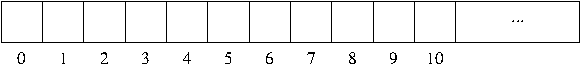
\includegraphics[keepaspectratio]{Pics/bytes}
\end{center}
\end{frame}

\begin{frame}
When a program is compiled, variables are mapped in some useful way to
memory location by the system (compiler and OS program loader)
\begin{itemize}
\item{So if we have a (4 byte) integer \code{n} in our code, the
  system might choose to place it at memory address 4 (a very unlikely place
  in real systems)}
\end{itemize}
\bigskip
\begin{center}
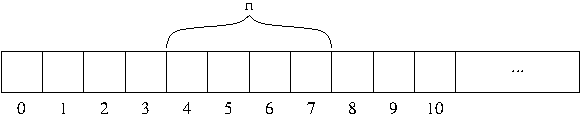
\includegraphics[keepaspectratio]{Pics/bytes2}
\end{center}
\end{frame}

\begin{frame}
Then every access of \code{n} in our code becomes a read or write of bytes 4--7
of memory
\begin{itemize}
\item{We say byte 4 is the {\em address\/} of the variable \code{n}}

\item{It's where the variable lives in memory}
\end{itemize}
\end{frame}

\begin{frame}
C gives us access to these addresses in our program: that is, we can find out
where a variable has been placed
\begin{itemize}
\item{Other languages might not reveal this kind of information,
  preferring to hide these details from the programmer}

\item{But for low-level programs that manipulate bits and bytes of
  memory this is just what they need}

\item{To get the address of a variable use the \code{\&} operator}
\end{itemize}
\end{frame}

\begin{frame}[fragile]
\begin{block}{}
\begin{lstlisting}
#include <stdio.h>
int main(void)
{
    int n = 1234;
    printf("n has value %d and address %p\n", n, &n);
    return 0; 
}
\end{lstlisting}
\end{block}
\begin{itemize}
\item{Produces\\
\code{n has value 1234 and address 0x7fff251f6d5c}}
\end{itemize}
\end{frame}

\begin{frame}
Note the difference between the {\em value\/} of \code{n} and the {\em
  address\/} of \code{n}
\begin{itemize}
\item{The value of \code{n} will always be 1234; the address
  (this example: 140732877607788 in decimal) will likely
  be different on different OSs, different on different compilers, possibly
  different on different runs on the same machine}

\item{It all depends on where in memory \code{n} happens to be placed
when the program is loaded to be run}
\end{itemize}
\end{frame}

\begin{frame}
\only<1>{But addresses are just integers}%
% \only<2->{{\LARGE Addresses are just integers}}
\begin{itemize}
\item{C does treat them slightly differently from normal integers to make
  certain nice things happen, but, at base, they are just integers}

\item{The \code{\%p} in \code{printf} prints addresses in hexadecimal,
  as that is often useful to the programmer}

% \item{Exercise. Compare \code{\%x} with \code{\%p}}
\end{itemize}
\end{frame}

\begin{frame}
Addresses are first-class values in C: this means you can use and manipulate
them just like any other values (like integers, doubles, etc.)
\begin{itemize}
\item{They are just integers, after all}

\item{Variables that hold addresses are called {\em pointer variables}}

\item{(Though it's not the variables that are pointers, but their
  values\dots)}
\end{itemize}
\end{frame}

\begin{frame}
So a pointer variable contains a simple integer (the address), but to make
things work nicely, C distinguishes between pointers and integers, and also
between pointers to different types
\begin{itemize}
\item{So a pointer to an integer is treated as different to a pointer to
  a double}

\item{And both are treated as different from a ordinary integer}

\item{This is a bit subtle: they are all simple integers underneath;
  it's just how the compiler {\em manipulates\/} those integers that will be
  different for different types}
\end{itemize}
\end{frame}

\begin{frame}
So the {\em interpretation\/} of that pointer integer is what is important
\begin{itemize}
\item{This is to make manipulations of them much more convenient}

\item{Now, memory doesn't ``know'' what kind of data is being
  stored at a particular address; memory is just a bunch of bytes}
\end{itemize}
\end{frame}

\begin{frame}
If I gave you \code{1000000010010010000111111011011} and asked
  ``what does that mean?'' you could legitimately say ``anything you like''
% IEEE single precision M_PI
\begin{itemize}
\item{It is purely the job of the program (and programmer) to
say what a particular bunch of bits is supposed to mean}

\item{The type of a variable or the type of a pointer encodes the
  information as to what bits they refer to ``mean''}

\item{Thus \code{int n = 99;} says ``allocate four bytes of memory
  somewhere and (while we access these bytes through this \code{n})
  interpret the bits in those bytes as an integer''}
\end{itemize}
\end{frame}

\begin{frame}
At one point the program might store an integer at a given address; later it
might store a double there
\begin{itemize}
\item{It is up to the program to interpret the bits at a given address
  in whatever way it wants}

\item{Don't make the mistake of assuming the computer magically
  ``knows'' what a bunch of bits means.  That's the job of the program}

\item{Note: while C makes this quite plain, the same is true for all
  computer languages}
\end{itemize}
\end{frame}

\begin{frame}[fragile]
We can declare pointer variables, e.g., \code{pn}

\begin{block}{}
\begin{lstlisting}
int n;
int *pn;
pn = &n;
\end{lstlisting}
\end{block}

The \code{*} is read as ``pointer to''; the variable \code{pn} has type
``pointer to \code{int}''
\begin{itemize}
\item{We also say ``\code{pn} is an \code{int} pointer''; sometimes
``\code{pn} is an integer reference'' or even ``\code{pn} is a reference to an
\code{int}''}

\item{``pointer to'' and ``reference to'' are the same as ``address of''}
\end{itemize}
\end{frame}

\begin{frame}[fragile]
In the opposite direction to \code{\&}, given a pointer value we can get at the
value stored at that address using the \code{*} operator
\begin{block}{}
\begin{lstlisting}
int n = 1234, *pn = &n; 

printf("n has value %d, pn has value %p\n", n, pn);
printf("the value pn points to is %d\n", *pn);
*pn = 23;
printf("n has value %d, pn has value %p\n", n, pn);
\end{lstlisting}
\end{block}
% \item{Produces}

\begin{block}{}
\begin{lstlisting}
n has value 1234, pn has value 0x7fff81aa38d4
the value pn points to is 1234
n has value 23, pn has value 0x7fff81aa38d4
\end{lstlisting}
\end{block}
\end{frame}

\begin{frame}
Initial values
\bigskip
\begin{center}
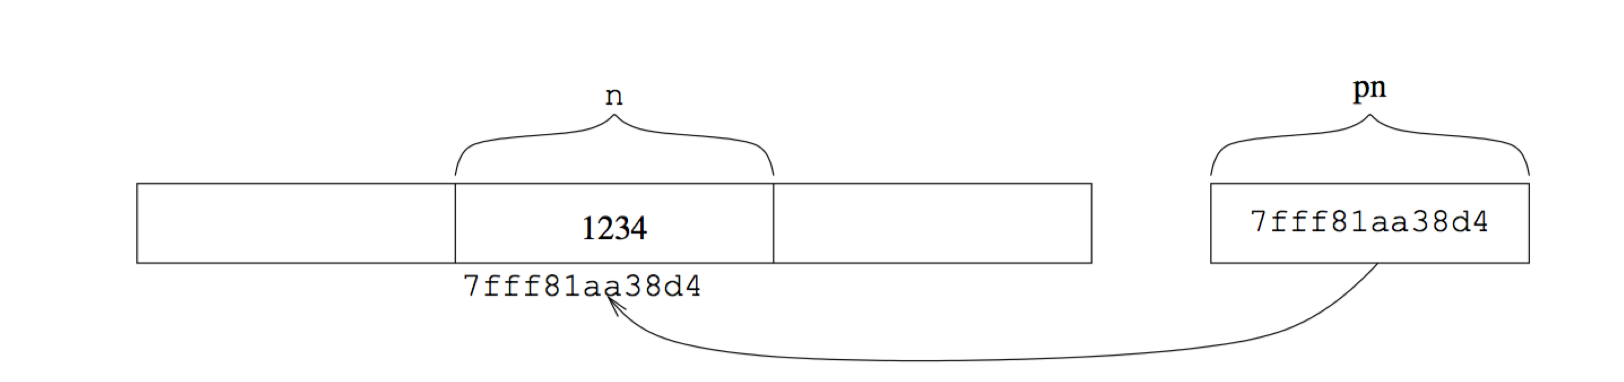
\includegraphics[height=3cm, keepaspectratio]{Pics/pointers1}
\end{center}
\end{frame}

\begin{frame}
After \code{*pn = 23}
\begin{center}
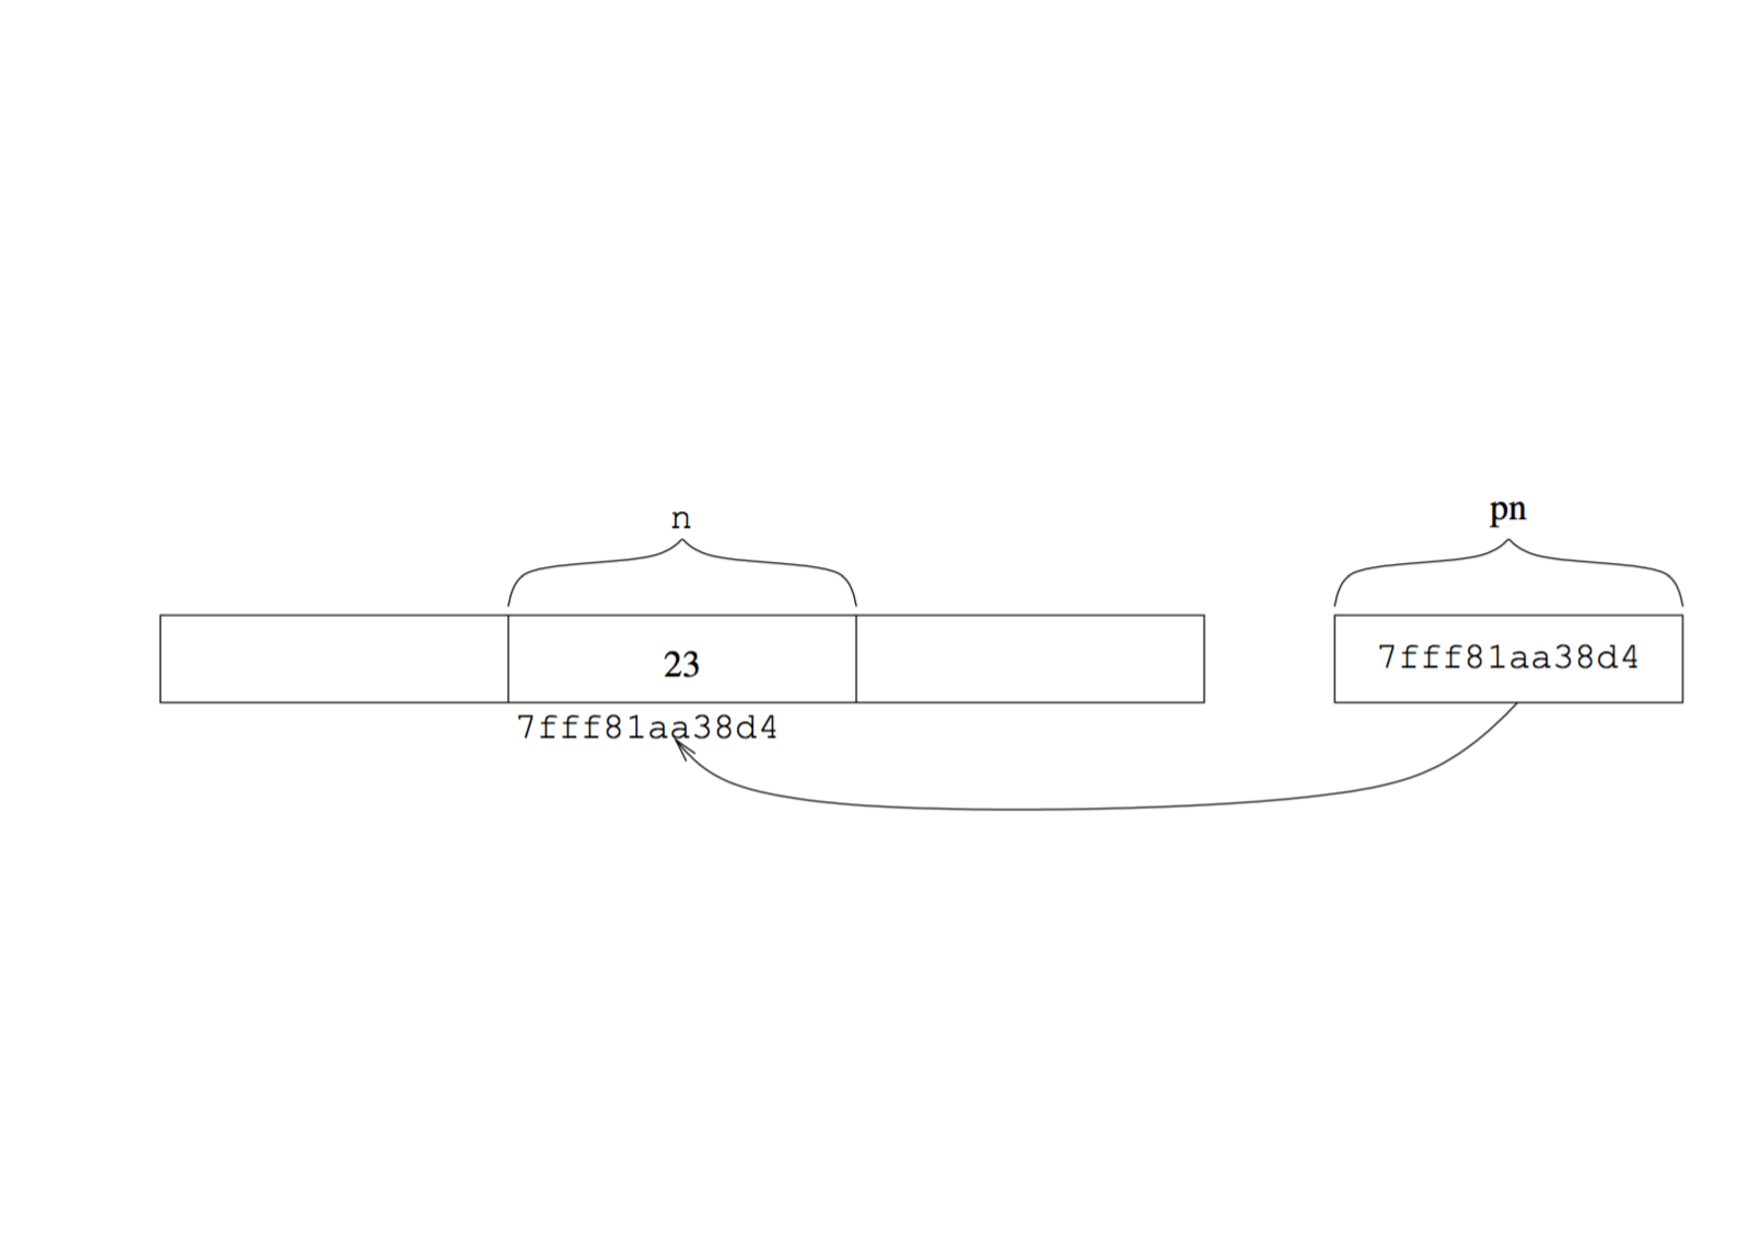
\includegraphics[height=3cm, keepaspectratio]{Pics/pointers2}
\end{center}
\end{frame}

\begin{frame}
\begin{center}
\textbf{Arrays and Pointers}
\end{center}
Pointers are intimately associated with arrays in C
\begin{itemize}
\item Consider an array \code{int a[4];}
\item In memory, C arrays are laid out simply
\end{itemize}
\begin{center}
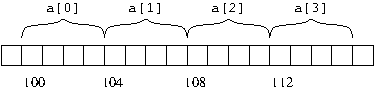
\includegraphics[height=2cm, keepaspectratio]{Pics/ptrarray1}
\end{center}
\bigskip
To be definite, we fix on using 4 byte (32 bit) integers
\end{frame}

\begin{frame}
In fact the variable \code{a} contains the address of the start of the array
\begin{center}
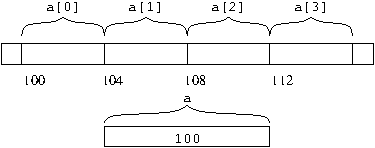
\includegraphics[height=3cm, keepaspectratio]{Pics/ptrarray2}
\end{center}
\begin{itemize}
\item{So \code{a} actually has type \code{int*} (with a caveat)}
\end{itemize}
\end{frame}

\begin{frame}

In the declarations of an array and a pointer\\
\code{int a[4];\\int *b;}\\
we need to be clear about what is happening
\begin{itemize}
\item{\code{a} is a variable of type pointer to integer {\bf and} a
  chunk of memory (e.g., 16 bytes) is reserved somewhere for the array; the
  value of the variable \code{a} will be the address of that chunk of memory}

\item{\code{b} is a variable of type pointer to integer, with no
  particular value, and no chunk of memory is reserved}
\end{itemize}
\end{frame}

\begin{frame}
\begin{center}
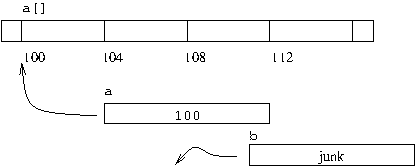
\includegraphics[height=3cm, keepaspectratio]{Pics/ptrarray3}
\end{center}

\code{int a[4]} sets up both \code{a} and the space for the array; \\
\code{int *b} just sets up \code{b}
\end{frame}

\begin{frame}
\code{b} is a pointer variable, so we can set its value: \code{b = a;}
\begin{center}
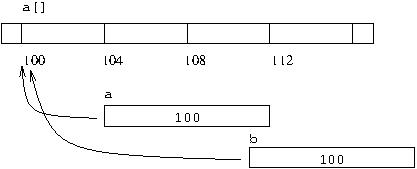
\includegraphics[height=3cm, keepaspectratio]{Pics/ptrarray4}
\end{center}
\begin{itemize}
\item{And now \code{b[1]} makes sense; it is the same as \code{a[1]}\\
\code{b[1]} is at address $100 + 1\times4 = 104$}
\end{itemize}
\end{frame}

\begin{frame}
We could equally do \code{b = a + 2}
\bigskip 
\begin{center}
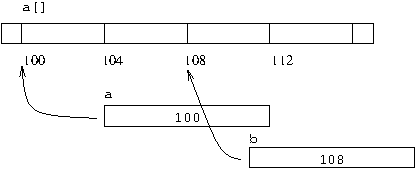
\includegraphics[height=3cm, keepaspectratio]{Pics/ptrarray5}
\end{center}
\begin{itemize}
\item{And now \code{b[1]} makes sense; it is the same as \code{a[3]}\\
\code{b[1]} is at address $108 + 1\times4 = 112$}

\item{And now \code{b[-1]} makes sense; it is the same as \code{a[1]}\\
\code{b[-1]} is at address $108 + (-1)\times4 = 104$}
\end{itemize}
\end{frame}

\begin{frame}
Another difference in this declaration is that \code{a} is a {\em constant\/}
variable (!)
\begin{itemize}
\item{We can't change the value of \code{a}}

\item{This is what we usually want from arrays: if we are thinking of
  \code{a} as indicating the start of an array we don't want its value
  wandering about in memory}

\item{And \code{b} is explicitly a variable pointer: if we need
  something variable, use a pointer}
\end{itemize}
\end{frame}

\begin{frame}[fragile]
\begin{block}{}
\begin{lstlisting}
void foo(void)
{
    int a[4];
    a++; 
}
\end{lstlisting}
\end{block}

gives an error message in the compiler

\end{frame}

\begin{frame}[fragile]
\begin{block}{}
\begin{lstlisting}
void foo(void)
{
    int a[4], *b = a;
    b++; 
}
\end{lstlisting}
\end{block}

is OK as \code{b} is allowed to vary
\end{frame}

\begin{frame}
\begin{center}
\textbf{Structures and Pointers}
\end{center}
Arrays are fixed-size structures in C
\begin{itemize}
\item Once declared, their length cannot be altered
\item Some languages allow variably sized arrays: there is a hidden cost to this, though, in speed of access to the elements of the array
\item Modern programs need dynamic structures, like lists and trees, that can grow and shrink
\item Lists and other dynamic datastructures are made easy in C by the use of structures and pointers
\end{itemize}
\end{frame}

\begin{frame}[fragile]
\begin{block}{}
\begin{lstlisting}
#include <stdio.h>

struct Stack
{
    int head;
    int max_size;
    int filo[1000];
};
\end{lstlisting}
\end{block}
\end{frame}

\begin{frame}[fragile]
We can define
\bigskip
\begin{block}{}
\begin{lstlisting}
struct IntList {
  int val;
  struct IntList *next;
};
\end{lstlisting}
\end{block}
\bigskip
This structure contains an integer value and a pointer to the next item in the list
\end{frame}

\begin{frame}[fragile]
We can define a few values
\bigskip
\begin{block}{}
\begin{lstlisting}
struct IntList a, b, c;
a.val = 12; a.next = &b;
b.val = 34; b.next = &c;
c.val = 56; c.next = 0;
\end{lstlisting}
\end{block}
\bigskip
N.B. this is not the right way to do this kind of thing
\begin{itemize}
\item So \code{a} is the head of the list; \code{b} is next; then \code{c}
\item We conventionally terminate the list with a 0 pointer as this turns out to be useful later (think about Boolean values)
\end{itemize}
\end{frame}

\begin{frame}[fragile]
Now the address values are distracting, not realistic and will vary depending on the compiler, runtime, and other factors.
\bigskip
\begin{itemize}
\item So the convention is to use box and pointer pictures. There are no particular values for the addresses, instead arrows indicate the relationships between the boxes
\item The actual locations of the structures in memory are not relevant here: but the relationships between the structures are
\end{itemize}
\begin{center}
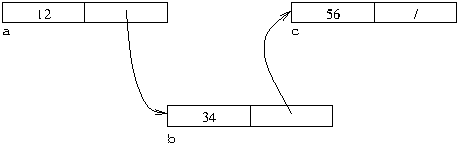
\includegraphics[height=3cm, keepaspectratio]{Pics/clist2}
\end{center}
\end{frame}

\begin{frame}[fragile]
Suppose we are given the head of the list, \code{a}
\bigskip
\begin{itemize}
\item Getting the value in \code{a} is easy: just \code{a.val}
\item How to get the next value in the list?
\item \code{a.next} is a pointer to \code{b}...
\item ... so we need \code{*(a.next)} to follow the pointer to get at the \code{struct b} ...
\item ... then \code{(*(a.next)).val} for the value in \code{b}
\end{itemize}
\end{frame}

\begin{frame}[fragile]
\begin{itemize}
\item This is ugly, but is such a common usage C provides the arrow \code{->} operator, to prettify code
\item So \code{expr->name} is the same as \code{(*expr).name}
\bigskip
\item Thus \code{a.next->val} same as \code{(*(a.next)).val} ,but easier to read
\item Further, \code{a.next->next->val} is the value in \code{c}
\item The first accessor is a dot, as \code{a} is a struct; the others are arrows as they follow pointers to structs
\end{itemize}
\end{frame}

\begin{frame}[fragile]
\begin{block}{}
\begin{lstlisting}
struct IntList {
  int val;
  struct IntList *next;
};

int main(){
    struct IntList a, b, c;
    a.val = 12; a.next = &b;
    b.val = 34; b.next = &c;
    c.val = 56; c.next = 0;
}
\end{lstlisting}
\end{block}
\end{frame}

\begin{frame}[fragile]
\begin{block}{}
\begin{lstlisting}
void printlist(struct intlist *l)
{
  struct IntList *ptr;
  for (ptr = l; ptr != NULL; ptr = ptr->next) {
     printf("%d\n", ptr->val);
  }
}
\end{lstlisting}
\end{block}
\end{frame}

\begin{frame}[fragile]
\begin{itemize}
\item We pass a pointer to the structure into \code{printlist}
\item The pointer variable \code{ptr} will iterate down the items in the list
\item The test for termination of loop is \code{ptr != NULL} as \code{ptr} is \code{NULL} at the end of the list
\item The \code{ptr} is updated at each iteration to point to the next item in the list
\end{itemize}
\end{frame}

\begin{frame}[fragile]
\begin{block}{}
\begin{lstlisting}
int main(){
    struct IntList a, b, c;
    a.val = 12; a.next = &b;
    b.val = 34; b.next = &c;
    c.val = 56; c.next = 0;
    
    printlist(&a);
}
\end{lstlisting}
\end{block}
\end{frame}

\begin{frame}[fragile]
We can also do this with recursion...
\begin{block}{}
\begin{lstlisting}
void printlistrec(struct IntList *l)
{
  if (l) {
    printf("%d\n", l->val);
    printlistrec(l->next);
  } 
}
\end{lstlisting}
\end{block}
\end{frame}

\section{Questions}

\end{document}









